\section{Leading checkpoint-delta directions are ablation-sensitive for measured refusal}
\label{sec:causal}

We next test whether leading spectral directions track refusal behavior. The
attention-output increment writes into the residual stream, which supports
geometric-overlap and ablation tests.

\paragraph{Setup.}
We form an empirical refusal direction $r_L$ as the difference of mean
last-token residual activations on harmful AdvBench \citep{zou2023universal}
and harmless Alpaca \citep{taori2023alpaca} prompts under the chat template,
following \citet{arditi2024}. Decoder blocks are zero-indexed. In the capture
sweep, block-$L$ \texttt{o\_proj} is paired with the residual after block $L$,
stored as \texttt{hidden\_states[L+1]}. At each block, we measure the fraction
of $r_L$ in the top-$k$ left-singular subspace of that block's
\texttt{o\_proj} increment and compare it with a random-$k$-subspace reference.
Because $r_L$ may encode harmfulness, style, and dataset differences alongside
refusal, the intervention claim concerns only a fixed substring-refusal score
on harmful prompts. Harmless-prompt effects, adaptive attacks, and human
judgments under the same intervention remain unmeasured.

\begin{figure}[t]
\centering
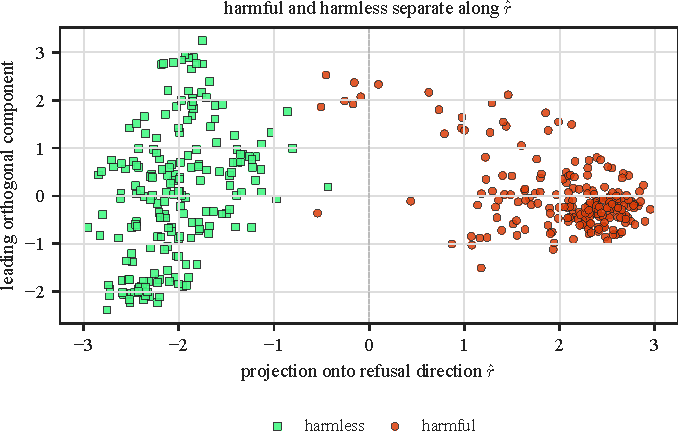
\includegraphics[width=0.58\textwidth]{../results/figures/geometry.pdf}
\caption{Last-token residual activations for harmful and harmless prompts,
projected onto the oriented refusal direction $\hat r$ (horizontal) and the
leading orthogonal component (vertical). Farther right means a larger
projection on $\hat r$; vertical position records the largest remaining
variation, not more refusal. The same observations define $\hat r$, the
orthogonal component, and the plotted points, so this is a construction view
rather than held-out separation.}
\label{fig:geometry}
\end{figure}

\paragraph{The refusal direction is enriched in leading spectral subspaces.}
At zero-indexed block $14$, the top-$8$ left-singular subspace of the
\texttt{o\_proj} increment, $8$ directions out of $4096$, captures $2.8\%$ of
the post-block refusal direction's squared norm, against a random-subspace
expectation of $0.20\%$: a $14.2\times$ enrichment ($n{=}256$ prompts per
class; Table~\ref{tab:capture}, Figure~\ref{fig:capture}). These values are
deterministic summaries of the fixed prompt set; Wilson intervals are reserved
for rate estimates below. Enrichment is $7.9\times$ at $k{=}16$ and
$3.7\times$ at $k{=}128$, so concentration is strongest near the top of the
spectrum. Across all $32$ blocks, top-$8$ enrichment exceeds the random
expectation in $31/32$ blocks, has median $4.6\times$, and peaks at
$14.2\times$. This supports an empirical association between the leading
checkpoint-delta subspace and the prompt-derived direction. It is not a
validation of the single-spike overlap formula in Section~\ref{sec:theory}.

\begin{table}[t]
\centering
\caption{Fraction of the post-block-$14$ refusal direction captured by the
top-$k$ left-singular subspace of the block-$14$ Base-to-Instruct
\texttt{o\_proj} increment. Values are deterministic summaries of the capture
analysis; Wilson intervals are used only for the rate estimates below.}
\label{tab:capture}
\small
\begin{tabular}{lccc}
\toprule
& $k=8$ & $k=32$ & $k=128$ \\
\midrule
\texttt{o\_proj} capture & $0.028$ & $0.050$ & $0.115$ \\
random-subspace reference & $0.002$ & $0.008$ & $0.031$ \\
\midrule
enrichment & $14.2\times$ & $6.4\times$ & $3.7\times$ \\
\bottomrule
\end{tabular}
\end{table}

\begin{figure}[t]
\centering
\begin{subfigure}{0.43\textwidth}
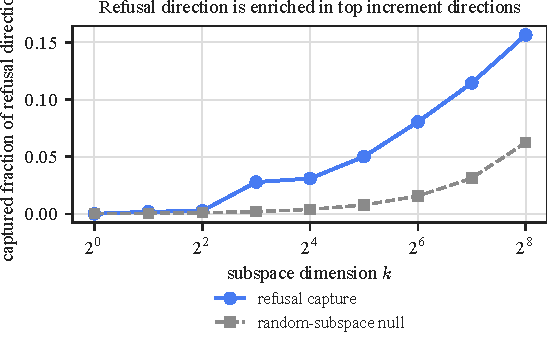
\includegraphics[width=\textwidth]{../results/figures/capture.pdf}
\end{subfigure}\hfill
\begin{subfigure}{0.55\textwidth}
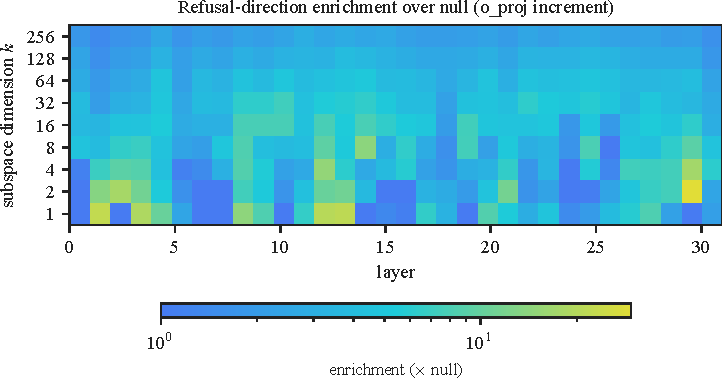
\includegraphics[width=\textwidth]{../results/figures/capture_heatmap.pdf}
\end{subfigure}
\caption{\emph{Left:} captured fraction of the post-block-$14$ refusal
direction by the top-$k$ block-$14$ \texttt{o\_proj} increment subspace and the
random reference. Rightward includes more directions; upward means more
capture. \emph{Right:} columns vary source block, rows vary $k$, and color gives
enrichment over random.}
\label{fig:capture}
\end{figure}

\paragraph{Global projection changes substring-scored refusal and capability.}
We project the top-$128$ left-singular subspace of the block-$14$
\texttt{o\_proj} increment out of the residual stream after every decoder
block. Applying one weight-derived basis globally tests model-wide dependence;
it does not localize a circuit. On the fixed $128$-prompt slice used for the
corrected audit, baseline substring refusal is $126/128=98.4\%$
($[94.5,99.6]\%$), spectral projection gives $18/128=14.1\%$
($[9.1,21.1]\%$), and one seeded random $128$-dimensional projection gives
$125/128=97.7\%$ ($[93.3,99.2]\%$). These are descriptive marginal Wilson
intervals, not an interval or test for either intervention contrast. The
corrected audit applies chat-formatted tokenization to all conditions. Earlier
full-$k$, source-block, rank-one, and steering runs used a different activation
or tokenization convention and are not used as evidence here.
Because refusal is substring-scored without an output-coherence gate, the
lower rate does not distinguish compliant answers from degenerate generations.

The same spectral intervention is highly destructive on capability benchmarks
(Figure~\ref{fig:ablation}). Baseline, spectral, and random-projection accuracy
is $65.4/41.8/54.4\%$ on MMLU, $80.0/50.2/65.8\%$ on ARC-C, and
$76.8/3.0/65.5\%$ on GSM8K
\citep{hendrycks2021mmlu,cobbe2021gsm8k,clark2018arc}. Thus the refusal change
is accompanied by broad capability loss, substantially larger than for this
random draw. One random subspace is a matched control, not a null distribution.
The experiment does not establish capability-preserving refusal removal.

\begin{figure}[t]
\centering
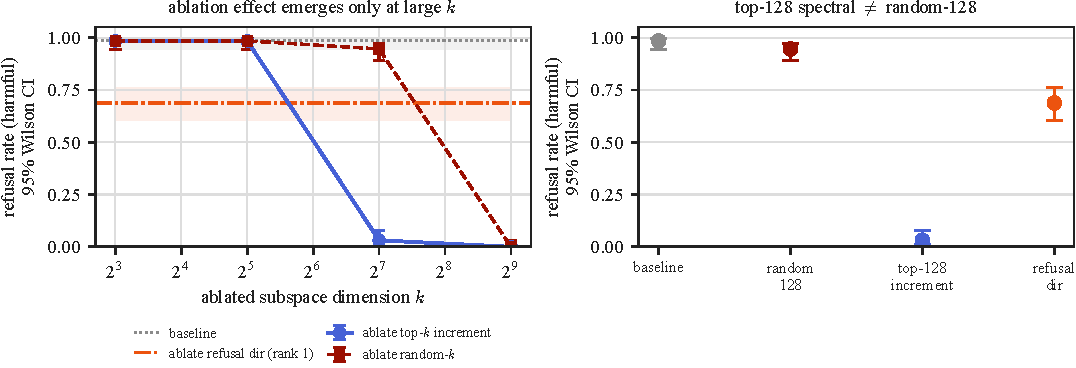
\includegraphics[width=0.96\textwidth]{../results/figures/ablation.pdf}
\caption{Corrected top-$128$ intervention audit. \emph{Left:}
substring-refusal rates on the same $128$ harmful prompts with descriptive
per-rate $95\%$ Wilson intervals; lower means fewer fixed refusal-phrase
matches. \emph{Right:} benchmark accuracy; higher is better. Spectral
projection reduces the refusal score but also causes substantially more
capability damage than the one seeded random projection.}
\label{fig:ablation}
\end{figure}
